\let\negmedspace\undefined
\let\negthickspace\undefined
\documentclass[12pt]{article}
\usepackage{cite}
\usepackage{float}
\usepackage{amsmath,amssymb,amsfonts,amsthm}
\usepackage{algorithmic}
\usepackage{graphicx}
\usepackage{textcomp}
\usepackage{xcolor}
\usepackage{txfonts}
\usepackage{listings}
\usepackage{enumitem}
\usepackage{mathtools}
\usepackage{gensymb}
\usepackage{comment}
\usepackage[breaklinks=true]{hyperref}
\usepackage{tkz-euclide} 
\usepackage{listings}
\usepackage{gvv}                                                             
\usepackage{gvv-book}     
\usepackage{xparse}
\usepackage{color}                                            
\usepackage{array}                                            
\usepackage{longtable}                                       
\usepackage{calc}                                             
\usepackage{multirow}
\usepackage{multicol}
\usepackage{hhline}                                           
\usepackage{ifthen}                                           
\usepackage{lscape}
\usepackage{tabularx}
\usepackage{array}
\usepackage{float}
\usepackage{geometry}
\geometry{left=1in, right=1in, top=1in, bottom=1in}

\begin{document}
\begin{center}
    {\LARGE \textbf{EC : ELECTRONICS AND COMMUNICATION ENGINEERING}}\\[0.7em]
    \begin{tabular}{c c}
        \textbf{Duration:} Three Hours & \textbf{Maximum Marks:} 100
    \end{tabular}
\end{center}

\textbf{Read the following instructions carefully}
\begin{enumerate}[leftmargin=2em,itemsep=0.5em]
    \item Do not open the seal of the Question Booklet until you are asked to do so by the invigilator.
    \item Take out the Optical Response Sheet (ORS) from this Question Booklet without breaking the seal and read the instructions printed on the ORS carefully. If you find that the Question Booklet Code printed at the right hand top corner of this page does not match with the Booklet Code on the ORS, exchange the booklet immediately with a new sealed Question Booklet.
    \item On the right half of the ORS, using ONLY a black ink ball point pen, (i) darken the bubble corresponding to your test paper code and the appropriate bubble under each digit of your registration number and (ii) write your registration number, your name and name of the examination centre and put your signature at the specified location.
    \item This Question Booklet contains \textbf{20 pages} including blank pages for rough work. After you are permitted to open the seal, please check all pages and report discrepancies, if any, to the invigilator.
    \item There are a total of \textbf{65 questions carrying 100 marks}. All these questions are of objective type. Each question has only one correct answer. Questions must be answered on the left hand side of the ORS by darkening the appropriate bubble (marked A, B, C, D) using ONLY a black ink ball point pen against the question number. For each question darken the bubble of the correct answer. More than one answer bubbled against a question will be treated as an incorrect response.
    \item Since bubbles darkened by the black ink ball point pen cannot be erased, candidates should darken the bubbles in the ORS very carefully.
    \item Questions Q.1 – Q.25 carry 1 mark each. Questions Q.26 – Q.55 carry 2 marks each. The 2-mark questions include two pairs of common data questions and two pairs of linked answer questions. The answer to the second question of the linked answer questions depends on the answer to the first question of the pair. If the first question in the linked pair is wrongly answered or is unattempted, then the answer to the second question in the pair will not be evaluated.
    \item Questions Q.56 – Q.65 belong to the General Aptitude (GA) section and carry a total of 15 marks. Questions Q.56 – Q.60 carry 1 mark each, and questions Q.61 – Q.65 carry 2 marks each.
    \item Unattempted questions will result in zero mark and wrong answers will result in \textbf{NEGATIVE marks}. For all 1 mark questions, $\tfrac{1}{3}$ mark will be deducted for each wrong answer. For all 2 mark questions, $\tfrac{2}{3}$ mark will be deducted for each wrong answer. However, in the case of the linked answer question pair, there will be negative marks only for wrong answer to the first question and no negative marks for wrong answer to the second question.
    \item Calculator is allowed whereas charts, graph sheets or tables are NOT allowed in the examination hall.
    \item Rough work can be done on the question paper itself. Blank pages are provided at the end of the question paper for rough work.
    \item Before the start of the examination, write your name and registration number in the space provided below using a black ink ball point pen.
\end{enumerate}

\newpage
\section*{Q.1 -- Q.25 carry one mark each.}
\begin{enumerate}[leftmargin=1.0em, label=\textbf{Q.\arabic*.}, itemsep=2em]

\item The current $i_b$ through the base of a silicon npn transistor is $i_b = 10000(\cos 1.01 \pi t + 1)$ mA. At 300 K, the $r_\pi$ in the small signal model of the transistor is

\noindent \textbf{[GATE EC 2012]}
\begin{figure}[H]\centering
\includegraphics[width=0.5\columnwidth]{figs/q1.png}
\caption{Power spectral density $S_X(\omega)$}
\label{fig:q1}
\end{figure}
\begin{multicols}{2}
    \begin{enumerate}
        \item $250~\Omega$
        \item $27.5~\Omega$
        \item $25~\Omega$
        \item $22.5~\Omega$
    \end{enumerate}
\end{multicols}

\item The power spectral density of a real process $X(t)$ for positive frequencies is shown below. The values of $E[X^2(t)]$ and $E[X(t)]$, respectively, are

\noindent \textbf{[GATE EC 2012]}
\begin{figure}[H]\centering
\includegraphics[width=0.5\columnwidth]{figs/q2.png}
\caption{Power spectral density $S_X(\omega)$}
\label{fig:q2}
\end{figure}
\begin{multicols}{2}
    \begin{enumerate}
        \item $6000/\pi, \; 0$
        \item $6400/\pi, \; 0$
        \item $6400/\pi, \; 20/(2\pi)$
        \item $6000/\pi, \; 20/(2\pi)$
    \end{enumerate}
\end{multicols}

\item In a baseband communications link, frequencies up to 3500 Hz are used for signaling. Using a raised cosine pulse with 75\% excess bandwidth and for no inter-symbol interference, the maximum possible signaling rate in symbols per second is

\noindent \textbf{[GATE EC 2012]}
\begin{multicols}{2}
    \begin{enumerate}
        \item 1750
        \item 2625
        \item 4000
        \item 5250
    \end{enumerate}
\end{multicols}

\item A plane wave propagating in air with 
\[
\vec{E} = (8\hat{a}_x + 6\hat{a}_y + 5\hat{a}_z) e^{j(3z+y+4x-\omega t)} \; \text{V/m}
\]
is incident on a perfectly conducting slab positioned at $x \leq 0$. The $\vec{E}$ field of the reflected wave is

\noindent \textbf{[GATE EC 2012]}
\begin{multicols}{2}
    \begin{enumerate}
        \item $( -8\hat{a}_x - 6\hat{a}_y - 5\hat{a}_z ) e^{j(3z+y-4x-\omega t)}$ V/m
        \item $( -8\hat{a}_x - 6\hat{a}_y + 5\hat{a}_z ) e^{j(3z+y-4x-\omega t)}$ V/m
        \item $( 8\hat{a}_x + 6\hat{a}_y + 5\hat{a}_z ) e^{j(3z+y-4x-\omega t)}$ V/m
        \item $( 8\hat{a}_x + 6\hat{a}_y - 5\hat{a}_z ) e^{j(3z+y-4x-\omega t)}$ V/m
    \end{enumerate}
\end{multicols}

\item The electric field of a uniform plane electromagnetic wave in free space, along the positive $x$ direction, is given by
\[
\vec{E} = 10(\hat{a}_y + j \hat{a}_z) e^{-j25x}
\]
The frequency and polarization of the wave, respectively, are
\noindent \textbf{[GATE EC 2012]}
\begin{multicols}{2}
    \begin{enumerate}
        \item 1.2 GHz and left circular
        \item 4 Hz and left circular
        \item 1.2 GHz and right circular
        \item 4 Hz and right circular
    \end{enumerate}
\end{multicols}

\item Consider the given circuit.

\noindent \textbf{[GATE EC 2012]}
\begin{figure}[H]\centering
\includegraphics[width=0.5\columnwidth]{figs/q6.png}
\caption{Circuit for Q.6}
\label{fig:q6}
\end{figure}
\begin{multicols}{2}
    \begin{enumerate}
        \item does not occur
        \item occurs when CLK = 0
        \item occurs when CLK = 1 and A = B = 1
        \item occurs when CLK = 1 and A = B = 0
    \end{enumerate}
\end{multicols}

\item The output $Y$ of a 2-bit comparator is logic 1 whenever the 2-bit input $A$ is greater than the 2-bit input $B$. The number of combinations for which the output is logic 1, is

\noindent \textbf{[GATE EC 2012]}
\begin{multicols}{2}
    \begin{enumerate}
        \item 4
        \item 6
        \item 8
        \item 10
    \end{enumerate}
\end{multicols}

\item The $i$–$v$ characteristics of the diode in the circuit given below are

\noindent \textbf{[GATE EC 2012]}
\begin{figure}[H]\centering
\includegraphics[width=0.5\columnwidth]{figs/q8.png}
\caption{Diode circuit for Q.8}
\label{fig:q8}
\end{figure}
\begin{multicols}{2}
    \begin{enumerate}
        \item 10 mA
        \item 9.3 mA
        \item 6.67 mA
        \item 6.2 mA
    \end{enumerate}
\end{multicols}

\item In the following figure, $C_1$ and $C_2$ are ideal capacitors. $C_1$ has been charged to 12 V before the ideal switch $S$ is closed at $t=0$. The current $i(t)$ for all $t$ is

\noindent \textbf{[GATE EC 2012]}
\begin{figure}[H]\centering
\includegraphics[width=0.5\columnwidth]{figs/q9.png}
\caption{Capacitor switching circuit for Q.9}
\label{fig:q9}
\end{figure}
\begin{multicols}{2}
    \begin{enumerate}
        \item zero
        \item a step function
        \item an exponentially decaying function
        \item an impulse function
    \end{enumerate}
\end{multicols}

\item The average power delivered to an impedance $(3-j4)\,\Omega$ by a current $i(t) = 5\cos(100\pi t + 100)$ A is

\noindent \textbf{[GATE EC 2012]}
\begin{multicols}{2}
    \begin{enumerate}
        \item 44.2 W
        \item 50 W
        \item 62.5 W
        \item 125 W
    \end{enumerate}
\end{multicols}

\item The unilateral Laplace transform of $f(t)$ is $\tfrac{1}{s^2+s+1}$. The unilateral Laplace transform of $t f(t)$ is

\noindent \textbf{[GATE EC 2012]}
\begin{multicols}{2}
    \begin{enumerate}
        \item $\dfrac{-s}{(s^2+s+1)^2}$
        \item $\dfrac{s+1}{(s^2+s+1)^2}$
        \item $\dfrac{s}{(s^2+s+1)^2}$
        \item $\dfrac{s+2}{(s^2+s+1)^2}$
    \end{enumerate}
\end{multicols}

\item With initial condition $x(1)=0.5$, the solution of the differential equation
\begin{align*}
\frac{dx}{dt} + x = t
\end{align*}
is

\noindent \textbf{[GATE EC 2012]}
\begin{multicols}{2}
    \begin{enumerate}
        \item $x = t - 1/2$
        \item $x = t - 2$
        \item $x = 2t$
        \item $x = t^2/2$
    \end{enumerate}
\end{multicols}

\item The diodes and capacitors in the circuit shown are ideal. The voltage $v(t)$ across the diode $D_1$ is

\noindent \textbf{[GATE EC 2012]}
\begin{figure}[H]\centering
\includegraphics[width=0.5\columnwidth]{figs/q13.png}
\caption{Circuit for Q.13}
\label{fig:q13}
\end{figure}
\begin{multicols}{2}
    \begin{enumerate}
        \item $\cos(\omega t) - 1$
        \item $\sin(\omega t)$
        \item $1 - \cos(\omega t)$
        \item $1 - \sin(\omega t)$
    \end{enumerate}
\end{multicols}

\item In the circuit shown

\noindent \textbf{[GATE EC 2012]}
\begin{figure}[H]\centering
\includegraphics[width=0.5\columnwidth]{figs/q14.png}
\caption{Logic circuit for Q.14}
\label{fig:q14}
\end{figure}
\begin{multicols}{2}
    \begin{enumerate}
        \item $Y = A + B + C$
        \item $Y = A(B+C)$
        \item $Y = (A+B)C$
        \item $Y = (A+C)B$
    \end{enumerate}
\end{multicols}

\item A source alphabet consists of $N$ symbols with the probability of the first two symbols being the same. A source encoder increases the probability of the first symbol by a small amount $\epsilon$ and decreases that of the second by $\epsilon$. After encoding, the entropy of the source

\noindent \textbf{[GATE EC 2012]}
\begin{multicols}{2}
    \begin{enumerate}
        \item increases
        \item remains the same
        \item increases only if $N=2$
        \item decreases
    \end{enumerate}
\end{multicols}

\item A coaxial cable with an inner diameter of 1 mm and outer diameter of 2.4 mm is filled with a dielectric of relative permittivity 10.89. Given $\mu_0 = 4\pi \times 10^{-7}$ H/m, $\epsilon_0 = 10^{-9}/(36\pi)$ F/m, the characteristic impedance of the cable is

\noindent \textbf{[GATE EC 2012]}
\begin{multicols}{2}
    \begin{enumerate}
        \item 330 $\Omega$
        \item 100 $\Omega$
        \item 143.3 $\Omega$
        \item 43.4 $\Omega$
    \end{enumerate}
\end{multicols}

\item The radiation pattern of an antenna in spherical coordinates is given by $F(\theta) = \cos^4\theta$ for $0 \leq \theta \leq \pi/2$. The directivity of the antenna is

\noindent \textbf{[GATE EC 2012]}
\begin{multicols}{2}
    \begin{enumerate}
        \item 10 dB
        \item 12.6 dB
        \item 11.5 dB
        \item 18 dB
    \end{enumerate}
\end{multicols}

\item If $x[n] = (1/2)^n u[n] - (1/3)^n u[n]$, then the region of convergence (ROC) of its $Z$-transform will be

\noindent \textbf{[GATE EC 2012]}
\begin{multicols}{2}
    \begin{enumerate}
        \item $|z| > 1/3$
        \item $1/3 < |z| < 1/2$
        \item $|z| > 1/2$
        \item $|z| < 1/3$
    \end{enumerate}
\end{multicols}

\item In the sum of products function $f(X,Y,Z) = \Sigma(2,3,4,5)$, the prime implicants are

\noindent \textbf{[GATE EC 2012]}
\begin{multicols}{2}
    \begin{enumerate}
        \item $XY, X'Y$
        \item $XY, X'Y, YZ$
        \item $XY, X'Y, Y'Z$
        \item $XY, X'Y, YZ, Y'Z$
    \end{enumerate}
\end{multicols}

\item A system with transfer function
\[
G(s) = \frac{s^2+9}{(s+1)(s+3)(s+4)}
\]
is excited by $\sin(\omega t)$. The steady-state output of the system is zero at

\noindent \textbf{[GATE EC 2012]}
\begin{multicols}{2}
    \begin{enumerate}
        \item $\omega = 1$ rad/s
        \item $\omega = 2$ rad/s
        \item $\omega = 3$ rad/s
        \item $\omega = 4$ rad/s
    \end{enumerate}
\end{multicols}

\item The impedance looking into nodes 1 and 2 in the given circuit is

\noindent \textbf{[GATE EC 2012]}
\begin{figure}[H]\centering
\includegraphics[width=0.5\columnwidth]{figs/q21.png}
\caption{Circuit for Q.21}
\label{fig:q21}
\end{figure}
\begin{multicols}{2}
    \begin{enumerate}
        \item 50 $\Omega$
        \item 100 $\Omega$
        \item 5 k$\Omega$
        \item 10.1 k$\Omega$
    \end{enumerate}
\end{multicols}

\item In the circuit shown below, the current through the inductor is

\noindent \textbf{[GATE EC 2012]}
\begin{figure}[H]\centering
\includegraphics[width=0.5\columnwidth]{figs/q22.png}
\caption{Circuit for Q.22}
\label{fig:q22}
\end{figure}
\begin{multicols}{2}
    \begin{enumerate}
        \item $\dfrac{1}{2+j}$ A
        \item $\dfrac{1}{1+j}$ A (with negative sign)
        \item $\dfrac{1}{1+j}$ A
        \item 0 A
    \end{enumerate}
\end{multicols}

\item Given
\[
f(z) = \frac{1}{(z+1)(z-1)(z+2)}
\]
If $C$ is a counterclockwise path in the $z$-plane such that $|z+1|=1$, the value of
\[
\frac{1}{2\pi j} \int_C f(z) \, dz
\]
is

\noindent \textbf{[GATE EC 2012]}
\begin{multicols}{2}
    \begin{enumerate}
        \item –2
        \item –1
        \item 1
        \item 2
    \end{enumerate}
\end{multicols}

\item Two independent random variables $X$ and $Y$ are uniformly distributed in the interval [–1, 1]. The probability that $\max[X,Y] < 1/2$ is

\noindent \textbf{[GATE EC 2012]}
\begin{multicols}{2}
    \begin{enumerate}
        \item 3/4
        \item 9/16
        \item 1/4
        \item 1/16
    \end{enumerate}
\end{multicols}

\item If $x = -1$, then the value of $x^x$ is

\noindent \textbf{[GATE EC 2012]}
\begin{multicols}{2}
    \begin{enumerate}
        \item $-e^{\pi/2}$
        \item $e^{\pi/2}$
        \item $x$
        \item 1
    \end{enumerate}
\end{multicols}

\newpage
\section*{Q.26 -- Q.55 carry two marks each.}
\begin{enumerate}[leftmargin=2.5em, label=\textbf{Q.\arabic*.}, itemsep=2em, start=26]

\item The source of a silicon ($n_i = 10^{10}$ per cm$^3$) n-channel MOS transistor has an area of 1 $\mu$m$^2$ and a depth of 1 $\mu$m. If the dopant density in the source is $10^{19}$/cm$^3$, the number of holes in the source region with the above volume is approximately

\noindent \textbf{[GATE EC 2012]}
\begin{multicols}{2}
    \begin{enumerate}
        \item $10^7$
        \item 100
        \item 10
        \item 0
    \end{enumerate}
\end{multicols}

\item A BPSK scheme operating over an AWGN channel with noise power spectral density $N_0/2$, uses equiprobable signals $s_1(t) = \sqrt{\tfrac{E}{T}} \sin(\omega_c t)$ and $s_2(t) = -\sqrt{\tfrac{E}{T}} \sin(\omega_c t)$ over the symbol interval $(0,T)$. If the local oscillator in a coherent receiver is ahead in phase by $45^\circ$ with respect to the received signal, the probability of error in the resulting system is

\noindent \textbf{[GATE EC 2012]}
\begin{multicols}{2}
    \begin{enumerate}
        \item $Q\!\left(\sqrt{\tfrac{E}{N_0}}\right)$
        \item $Q\!\left(\sqrt{\tfrac{E}{2N_0}}\right)$
        \item $Q\!\left(\sqrt{\tfrac{E}{4N_0}}\right)$
        \item $Q\!\left(\sqrt{\tfrac{E}{N_0/2}}\right)$
    \end{enumerate}
\end{multicols}

\item A transmission line with a characteristic impedance of 100 $\Omega$ is used to match a 50 $\Omega$ section to a 200 $\Omega$ section. If the matching is to be done both at 429 MHz and 1 GHz, the length of the transmission line can be approximately

\noindent \textbf{[GATE EC 2012]}
\begin{multicols}{2}
    \begin{enumerate}
        \item 82.5 cm
        \item 1.05 m
        \item 1.58 m
        \item 1.75 m
    \end{enumerate}
\end{multicols}

\item The input $x(t)$ and output $y(t)$ of a system are related as
\begin{align*}
y(t) = \int_{-\infty}^{t} x(\tau)\cos(3\tau) \, d\tau
\end{align*}
The system is

\noindent \textbf{[GATE EC 2012]}
\begin{multicols}{2}
    \begin{enumerate}
        \item time-invariant and stable
        \item stable and not time-invariant
        \item time-invariant and not stable
        \item not time-invariant and not stable
    \end{enumerate}
\end{multicols}

\item The feedback system shown below oscillates at $2$ rad/s when

\noindent \textbf{[GATE EC 2012]}
\begin{figure}[H]\centering
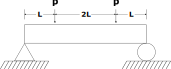
\includegraphics[width=0.5\columnwidth]{figs/q30.png}
\caption{Feedback system for Q.30}
\label{fig:q30}
\end{figure}
\begin{multicols}{2}
    \begin{enumerate}
        \item $K=2, \; a=0.75$
        \item $K=3, \; a=0.75$
        \item $K=4, \; a=0.5$
        \item $K=2, \; a=0.5$
    \end{enumerate}
\end{multicols}

\item The Fourier transform of a signal $h(t)$ is
\[
H(\omega) = \frac{2\sin(2\omega)}{\omega}\cos(\omega)
\]
The value of $h(0)$ is

\noindent \textbf{[GATE EC 2012]}
\begin{multicols}{2}
    \begin{enumerate}
        \item 1/4
        \item 1/2
        \item 1
        \item 2
    \end{enumerate}
\end{multicols}

\item The state variable description of an LTI system is given by
\begin{align*}
\myvec{
\dot{x}_1 \\ \dot{x}_2 \\ \dot{x}_3
}
&=
\myvec{
0 & 0 & a_1 \\
0 & 0 & a_2 \\
0 & 0 & a_3
}
\myvec{
x_1 \\ x_2 \\ x_3
}
+
\myvec{
1 \\ 0 \\ 0
} u
\\[0.5em]
y &=
\myvec{
0 & 0 & 1
}
\myvec{
x_1 \\ x_2 \\ x_3
}
\end{align*}

The system is controllable for

\noindent \textbf{[GATE EC 2012]}
\begin{multicols}{2}
    \begin{enumerate}
        \item $a_1 \neq 0, \; a_2 = 0, \; a_3 \neq 0$
        \item $a_1 = 0, \; a_2 \neq 0, \; a_3 \neq 0$
        \item $a_1 = 0, \; a_2 \neq 0, \; a_3 = 0$
        \item $a_1 \neq 0, \; a_2 \neq 0, \; a_3 = 0$
    \end{enumerate}
\end{multicols}

\item Assuming both the voltage sources are in phase, the value of $R$ for which maximum power is transferred from circuit A to circuit B is

\noindent \textbf{[GATE EC 2012]}
\begin{figure}[H]\centering
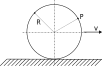
\includegraphics[width=0.5\columnwidth]{figs/q33.png}
\caption{Circuit for Q.33}
\label{fig:q33}
\end{figure}
\begin{multicols}{2}
    \begin{enumerate}
        \item 0.8 $\Omega$
        \item 1.4 $\Omega$
        \item 2 $\Omega$
        \item 2.8 $\Omega$
    \end{enumerate}
\end{multicols}

\item Consider the differential equation
\begin{align*}
\frac{d^2y(t)}{dt^2} + \frac{dy(t)}{dt} + y(t) &= t, \quad y(0)=-2, \; y'(0)=0
\end{align*}
The numerical value of $y'(0^+)$ is

\noindent \textbf{[GATE EC 2012]}
\begin{multicols}{2}
    \begin{enumerate}
        \item –2
        \item –1
        \item 0
        \item 1
    \end{enumerate}
\end{multicols}

\item The direction of vector $\vec{A}$ is radially outward from the origin, with $\vec{A} = k r^n \hat{r}$, where $r = \sqrt{x^2+y^2+z^2}$ and $k$ is a constant. The value of $n$ for which $\nabla \cdot \vec{A} = 0$ is

\noindent \textbf{[GATE EC 2012]}
\begin{multicols}{2}
    \begin{enumerate}
        \item –2
        \item 2
        \item 1
        \item 0
    \end{enumerate}
\end{multicols}

\item A fair coin is tossed till a head appears for the first time. The probability that the number of required tosses is odd, is

\noindent \textbf{[GATE EC 2012]}
\begin{multicols}{2}
    \begin{enumerate}
        \item 1/3
        \item 1/2
        \item 2/3
        \item 3/4
    \end{enumerate}
\end{multicols}

\item In the CMOS circuit shown, electron and hole mobilities are equal, and M1 and M2 are equally sized. The device M1 is in the linear region if

\noindent \textbf{[GATE EC 2012]}
\begin{figure}[H]\centering
\includegraphics[width=0.5\columnwidth]{figs/q37.png}
\caption{CMOS circuit for Q.37}
\label{fig:q37}
\end{figure}
\begin{multicols}{2}
    \begin{enumerate}
        \item $V_{in} < 1.875$ V
        \item $1.875 < V_{in} < 3.125$ V
        \item $V_{in} > 3.125$ V
        \item $0 < V_{in} < 5$ V
    \end{enumerate}
\end{multicols}

\item A binary symmetric channel (BSC) has a transition probability of $1/8$. If the binary transmit symbol $X$ is such that $P(X=0)=9/10$, then the probability of error for an optimum receiver will be

\noindent \textbf{[GATE EC 2012]}
\begin{multicols}{2}
    \begin{enumerate}
        \item 7/80
        \item 63/80
        \item 9/10
        \item 1/10
    \end{enumerate}
\end{multicols}

\item The signal $m(t)$ as shown is applied both to a phase modulator (with $k_p$ as the phase constant) and a frequency modulator (with $k_f$ as the frequency constant) having the same carrier frequency. The ratio $k_p/k_f$ (in rad/Hz) for the same maximum phase deviation is

\noindent \textbf{[GATE EC 2012]}
\begin{figure}[H]\centering
\includegraphics[width=0.5\columnwidth]{figs/q39.png}
\caption{Signal $m(t)$ for Q.39}
\label{fig:q39}
\end{figure}
\begin{multicols}{2}
    \begin{enumerate}
        \item $8\pi$
        \item $4\pi$
        \item $2\pi$
        \item $\pi$
    \end{enumerate}
\end{multicols}

\item The magnetic field along the propagation direction inside a rectangular waveguide with the cross-section shown in the figure is
\[
H_z = 3 \cos(2.94\times 10^{10} x)\cos(6.18\times 10^{10} y)\cos(8.36\times 10^{10} z - \beta z)
\]
The phase velocity $v_p$ of the wave inside the waveguide satisfies

\noindent \textbf{[GATE EC 2012]}
\begin{figure}[H]\centering
\includegraphics[width=0.5\columnwidth]{figs/q40.png}
\caption{Waveguide cross-section for Q.40}
\label{fig:q40}
\end{figure}
\begin{multicols}{2}
    \begin{enumerate}
        \item $v_p > c$
        \item $v_p = c$
        \item $v_p < c$
        \item $v_p = 0$
    \end{enumerate}
\end{multicols}

\item The circuit shown is a

\noindent \textbf{[GATE EC 2012]}
\begin{figure}[H]\centering
\includegraphics[width=0.5\columnwidth]{figs/q41.png}
\caption{Circuit for Q.41}
\label{fig:q41}
\end{figure}
\begin{multicols}{2}
    \begin{enumerate}
        \item low pass filter with $f_{3dB} = \tfrac{1}{C(R_1+R_2)}$ rad/s
        \item high pass filter with $f_{3dB} = \tfrac{1}{CR_1}$ rad/s
        \item low pass filter with $f_{3dB} = \tfrac{1}{CR_1}$ rad/s
        \item high pass filter with $f_{3dB} = \tfrac{1}{C(R_1+R_2)}$ rad/s
    \end{enumerate}
\end{multicols}

\item Let $y[n]$ denote the convolution of $h[n]$ and $g[n]$, where $h[n] = (1/2)^n u[n]$ and $g[n]$ is a causal sequence. If $y[0]=1$ and $y[1]=1/2$, then $g[1]$ equals

\noindent \textbf{[GATE EC 2012]}
\begin{multicols}{2}
    \begin{enumerate}
        \item 0
        \item 1/2
        \item 1
        \item 3/2
    \end{enumerate}
\end{multicols}

\item The state transition diagram for the logic circuit shown is

\noindent \textbf{[GATE EC 2012]}
\begin{figure}[H]\centering
\includegraphics[width=0.5\columnwidth]{figs/q43.png}
\caption{Logic circuit for Q.43}
\label{fig:q43}
\end{figure}
\begin{multicols}{2}
    \begin{enumerate}
        \item Diagram A
        \item Diagram B
        \item Diagram C
        \item Diagram D
    \end{enumerate}
\end{multicols}

\item The voltage gain $A_v$ of the circuit shown below is

\noindent \textbf{[GATE EC 2012]}
\begin{figure}[H]\centering
\includegraphics[width=0.5\columnwidth]{figs/q44.png}
\caption{Amplifier circuit for Q.44}
\label{fig:q44}
\end{figure}
\begin{multicols}{2}
    \begin{enumerate}
        \item $A_v \approx 200$
        \item $A_v \approx 100$
        \item $A_v \approx 20$
        \item $A_v \approx 10$
    \end{enumerate}
\end{multicols}

\item If $V_A = -6$ V and $V_B = V$, then $V_D - V_C$ is

\noindent \textbf{[GATE EC 2012]}
\begin{figure}[H]\centering
\includegraphics[width=0.5\columnwidth]{figs/q45.png}
\caption{Circuit for Q.45}
\label{fig:q45}
\end{figure}
\begin{multicols}{2}
    \begin{enumerate}
        \item –5 V
        \item 2 V
        \item 3 V
        \item 6 V
    \end{enumerate}
\end{multicols}


\end{enumerate}

\newpage
\section*{Q.46 -- Q.65}
\begin{enumerate}[leftmargin=2.5em, label=\textbf{Q.\arabic*.}, itemsep=2em, start=46]

\item The maximum value of
\[
f(x) = x^{3} - 9x^{2} + 24x + 5
\]
in the interval $[1,6]$ is
\noindent \textbf{[GATE EC 2012]}
\begin{multicols}{2}
    \begin{enumerate}[label=\alph*.]
        \item 21
        \item 25
        \item 41
        \item 46
    \end{enumerate}
\end{multicols}

\item Given that
\[
A = \begin{pmatrix}-5 & -3\\[4pt] 2 & 0\end{pmatrix}, \qquad
I = \begin{pmatrix}1 & 0\\[4pt] 0 & 1\end{pmatrix},
\]
the value of $A^{3}$ is
\noindent \textbf{[GATE EC 2012]}
\begin{multicols}{2}
    \begin{enumerate}[label=\alph*.]
        \item $15A + 12I$
        \item $19A + 30I$
        \item $17A + 15I$
        \item $17A + 21I$
    \end{enumerate}
\end{multicols}

\item[] \textbf{Common data for Questions 48 and 49:}\\

With 10 V dc connected at port A in the linear non-reciprocal two-port network shown below, the following were observed:
\begin{enumerate}[leftmargin=*, itemsep=0.2em]
    \item 1 $\Omega$ connected at port B draws a current of 3 A.
    \item 2.5 $\Omega$ connected at port B draws a current of 2 A.
\end{enumerate}

\begin{figure}[H]\centering
\includegraphics[width=0.5\columnwidth]{figs/q48.png}
\caption{Two-port network (common data for Q.48 and Q.49)}
\label{fig:q48}
\end{figure}

\item With 10 V dc at port A, the current drawn by 7 $\Omega$ connected at port B is
\noindent \textbf{[GATE EC 2012]}
\begin{multicols}{2}
    \begin{enumerate}[label=\alph*.]
        \item $3/7$ A
        \item $5/7$ A
        \item 1 A
        \item $9/7$ A
    \end{enumerate}
\end{multicols}

\item For the same network (common data), if 6 V dc is connected at port A, 1 $\Omega$ at port B draws $7/3$ A. If 8 V dc is connected to port A, the open-circuit voltage at port B is
\noindent \textbf{[GATE EC 2012]}
\begin{multicols}{2}
    \begin{enumerate}[label=\alph*.]
        \item 6 V
        \item 7 V
        \item 8 V
        \item 9 V
    \end{enumerate}
\end{multicols}

\item[] \textbf{Common data for Questions 50 and 51:}\\

(Three-dimensional view of an n-channel MOS transistor; $d=20\,$nm, width $=1\ \mu$m; depletion width at every p–n junction $=10\,$nm; relative permittivities: Si $=11.7$, SiO$_2=3.9$, $\varepsilon_0 = 8.9\times10^{-12}$ F/m.)

\begin{figure}[H]\centering
\includegraphics[width=0.5\columnwidth]{figs/q50.png}
\caption{3D view of MOS transistor (common data for Q.50 and Q.51)}
\label{fig:q50}
\end{figure}

\item The gate–source overlap capacitance is approximately

\noindent \textbf{[GATE EC 2012]}
\begin{multicols}{2}
    \begin{enumerate}[label=\alph*.]
        \item $0.7\ \text{fF}$
        \item $0.7\ \text{pF}$
        \item $0.35\ \text{fF}$
        \item $0.24\ \text{pF}$
    \end{enumerate}
\end{multicols}

\item The source–body junction capacitance is approximately

\noindent \textbf{[GATE EC 2012]}
\begin{multicols}{2}
    \begin{enumerate}[label=\alph*.]
        \item $2\ \text{fF}$
        \item $7\ \text{fF}$
        \item $2\ \text{pF}$
        \item $7\ \text{pF}$
    \end{enumerate}
\end{multicols}

\item[] \textbf{Linked answer questions 52 and 53 (statement):}\\

An infinitely long uniform solid wire of radius $a$ carries a uniform DC current density $\mathbf{j}$.  

\item The magnetic field at a distance $r$ from the center of the wire is proportional to

\noindent \textbf{[GATE EC 2012]}
\begin{multicols}{2}
    \begin{enumerate}[label=\alph*.]
        \item $r$ for $r<a$ and $1/r^{2}$ for $r>a$
        \item $0$ for $r<a$ and $1/r$ for $r>a$
        \item $r$ for $r<a$ and $1/r$ for $r>a$
        \item $0$ for $r<a$ and $1/r^{2}$ for $r>a$
    \end{enumerate}
\end{multicols}

\item A hole of radius $b$ ($b<a$) is drilled along the length of the wire at a distance $d$ from the center (see figure). The magnetic field inside the hole is

\noindent \textbf{[GATE EC 2012]}
\begin{figure}[H]\centering
\includegraphics[width=0.5\columnwidth]{figs/q53.png}
\caption{Cross-section for Q.53 (hole in wire)}
\label{fig:q53}
\end{figure}
\begin{multicols}{2}
    \begin{enumerate}[label=\alph*.]
        \item uniform and depends only on $d$
        \item uniform and depends only on $b$
        \item uniform and depends on both $b$ and $d$
        \item non-uniform
    \end{enumerate}
\end{multicols}

\item[] \textbf{Statement for Linked Answer Questions 54 and 55:}\\
The transfer function of a compensator is given by
\[
G_c(s)=\frac{bs+1}{as+1}.
\]

\item $G_c(s)$ is a lead compensator if

\noindent \textbf{[GATE EC 2012]}
\begin{multicols}{2}
    \begin{enumerate}[label=\alph*.]
        \item $a=1,\ b=2$
        \item $a=3,\ b=2$
        \item $a=-3,\ b=-1$
        \item $a=3,\ b=1$
    \end{enumerate}
\end{multicols}

\item The phase of the above lead compensator is maximum at

\noindent \textbf{[GATE EC 2012]}
\begin{multicols}{2}
    \begin{enumerate}[label=\alph*.]
        \item $2\ \text{rad/s}$
        \item $3^{1/2}\ \text{rad/s}$
        \item $6^{1/2}\ \text{rad/s}$
        \item $1/3\ \text{rad/s}$
    \end{enumerate}
\end{multicols}

\item[] \textbf{General Aptitude (GA) — Q.56–Q.65 (compulsory). Q.56–Q.60 carry 1 mark each; Q.61–Q.65 carry 2 marks each.}

\item If $(1.001)^{1259}=3.52$ and $(1.001)^{2062}=7.85$, then $(1.001)^{3321}=$

\noindent \textbf{[GATE EC 2012]}
\begin{multicols}{2}
    \begin{enumerate}[label=\alph*.]
        \item 2.23
        \item 4.33
        \item 11.37
        \item 27.64
    \end{enumerate}
\end{multicols}

\item Choose the most appropriate alternative to complete the sentence:
\[
\text{If the tired soldier wanted to lie down, he \_\_\_ the mattress out on the balcony.}
\]

\noindent \textbf{[GATE EC 2012]}
\begin{multicols}{2}
    \begin{enumerate}[label=\alph*.]
        \item should take
        \item shall take
        \item should have taken
        \item will have taken
    \end{enumerate}
\end{multicols}

\item Choose the most appropriate word to complete the sentence:

\[
\text{Given the seriousness of the situation that he had to face, his \_\_\_ was impressive.}
\]

\noindent \textbf{[GATE EC 2012]}
\begin{multicols}{2}
    \begin{enumerate}[label=\alph*.]
        \item beggary
        \item nomenclature
        \item jealousy
        \item nonchalance
    \end{enumerate}
\end{multicols}

\item Which one of the following options is the closest in meaning to the word \textbf{Latitude}?

\noindent \textbf{[GATE EC 2012]}
\begin{multicols}{2}
    \begin{enumerate}[label=\alph*.]
        \item Eligibility
        \item Freedom
        \item Coercion
        \item Meticulousness
    \end{enumerate}
\end{multicols}

\item One of the parts (A, B, C, D) in the sentence given below contains an ERROR. Which one is INCORRECT?

\emph{I requested that he should be given the driving test today instead of tomorrow.}

\noindent \textbf{[GATE EC 2012]}
\begin{multicols}{2}
    \begin{enumerate}[label=\alph*.]
        \item requested that
        \item should be given
        \item the driving test
        \item instead of tomorrow
    \end{enumerate}
\end{multicols}

\item One of the legacies of the Roman legions was discipline. (Passage-based question — choose best summary statement.)

\noindent \textbf{[GATE EC 2012]}
\begin{multicols}{2}
    \begin{enumerate}[label=\alph*.]
        \item Thorough regimentation was the main reason for the efficiency of the Roman legions even in adverse circumstances.
        \item The legions were treated inhumanly as if the men were animals.
        \item Discipline was the armies’ inheritance from their seniors.
        \item The harsh discipline to which the legions were subjected led to the odds and conditions being against them.
    \end{enumerate}
\end{multicols}

\item Raju has 14 currency notes in his pocket consisting only of Rs.20 and Rs.10 notes. The total value is Rs.230. The number of Rs.10 notes Raju has is

\noindent \textbf{[GATE EC 2012]}
\begin{multicols}{2}
    \begin{enumerate}[label=\alph*.]
        \item 5
        \item 6
        \item 9
        \item 10
    \end{enumerate}
\end{multicols}

\item There are eight indistinguishable bags of rice; seven have equal weight and one is slightly heavier. Using a weighing balance of unlimited capacity, the minimum number of weighings required to identify the heavier bag is

\noindent \textbf{[GATE EC 2012]}
\begin{multicols}{2}
    \begin{enumerate}[label=\alph*.]
        \item 2
        \item 3
        \item 4
        \item 8
    \end{enumerate}
\end{multicols}

\item The data below summarize monthly budget (Rs.) — Food: 4000; Clothing: 1200; Rent: 2000; Savings: 1500; Other expenses: 1800. The approximate percentage of the monthly budget NOT spent on savings is

\noindent \textbf{[GATE EC 2012]}
\begin{multicols}{2}
    \begin{enumerate}[label=\alph*.]
        \item 10\%
        \item 14\%
        \item 81\%
        \item 86\%
    \end{enumerate}
\end{multicols}

\item A and B decide to meet between 1 PM and 2 PM. Whoever arrives first will not wait more than 15 minutes. The probability they meet is

\noindent \textbf{[GATE EC 2012]}
\begin{multicols}{2}
    \begin{enumerate}[label=\alph*.]
        \item $1/4$
        \item $1/16$
        \item $7/16$
        \item $9/16$
    \end{enumerate}
\end{multicols}

\end{enumerate}

\end{enumerate}

\end{document}
